\documentclass{beamer}
\usetheme{Boadilla}
\usepackage[thinc]{esdiff}
\usepackage{siunitx}
\usepackage{booktabs}
\usepackage{xcolor}
\usepackage{transparent}
\usepackage{graphicx}
\usepackage{subcaption}
\usepackage{tikz}
\usepackage[x11names]{xcolor}

\setbeamertemplate{bibliography item}[text]
\bibliographystyle{apalike}
\newcommand{\backupbegin}{
   \newcounter{finalframe}
   \setcounter{finalframe}{\value{framenumber}}
}
\newcommand{\backupend}{
   \setcounter{framenumber}{\value{finalframe}}
}


\setbeamertemplate{frametitle}[default][center]

\subtitle{}
\title{}
%\titlegraphic{\includegraphics[width=0.9\linewidth,height=0.4\linewidth]{image.png}}
\author{Ole Merkes}
\institute{University of Hamburg}
\date{\today}


\AtBeginSection[]
{
    \begin{frame}
        %\frametitle{Table of Contents}
        \tableofcontents[currentsection,currentsubsection]
    \end{frame}
}

\begin{document}

% \setbeamertemplate{background canvas}{
% \transparent{0.4}\includegraphics[width=\paperwidth,height=\paperheight]{image.png}
% }%
\begin{frame}
    \titlepage
\end{frame}
%\setbeamertemplate{background canvas}[default]


\begin{frame}
    \frametitle{Scaling of the HC}
    \begin{block}{Angular momentum conserving}  
    \begin{align}
        \Phi_H\sim&\left(\frac{gH\Delta_h}{\Omega^2R_E^2}\right)^{1/2}\\
        \psi_\mathrm{max} \sim & \frac{1}{\tau}\frac{g^{3/2}(H\Delta_h)^{5/2}}{\Omega^3R_E^2\Delta_v}
    \end{align}
    \end{block}
    \begin{block}{Baroclinic instability and eddy flux}
        \begin{align}
            \theta_C \sim& \left(\frac{NH}{2\Omega a}\right)^{1/2}\\
            \psi(1-Ro)\approx& \frac{S}{f}
        \end{align}
    \end{block}
\end{frame}

\begin{frame}
    \frametitle{ECHAM mean meridional circulation}
    \begin{figure}
        \centering
        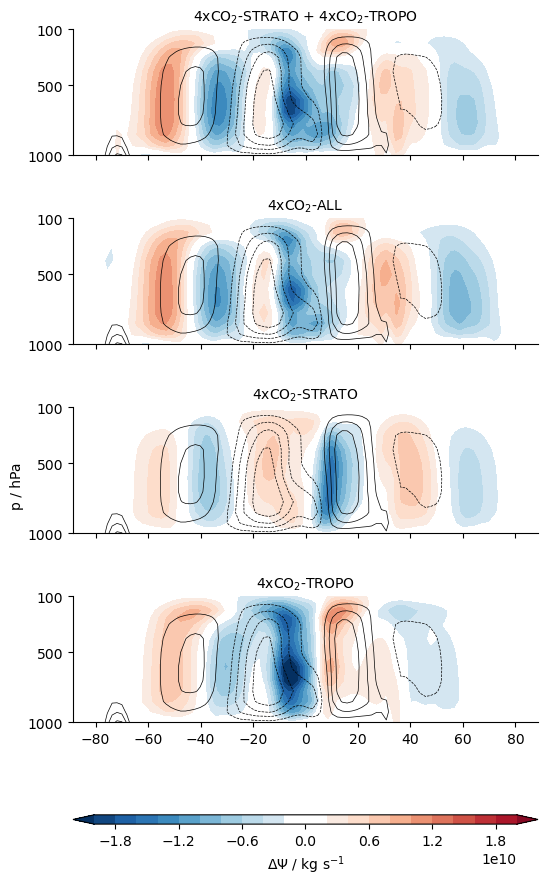
\includegraphics[height=\textheight]{figures/circulation_echam.png}
    \end{figure}
\end{frame}

\begin{frame}
    \frametitle{Definitions D'Agostino et al. 2017}
    \begin{itemize}
        \item meridional near-surface(averaged between the 700 and 800 hPa levels) potential
        temperature contrast $\Delta_h\theta(p,\varphi)=\Bar{\theta}(800-700\;\si{hPa},0-10\;\unit{\degree})-\Bar{\theta}(800-700\;\si{hPa},40-60\;\si{\degree})$
        \item subtropical near-surface static stability $\Delta_v\theta(p,\varphi)=\Bar{\theta}(700\;\si{hPa},20-40\;\unit{\degree})-\Bar{\theta}(800\;\si{hPa},20-40\;\si{\degree})$
        \item tropical tropopause pressure height $p_t(\varphi)=\Bar{p}(15\unit{\degree S}- 15\unit{\degree N})$ 
        \item extratropical tropopause height $p_{et}(\varphi)=\Bar{p}(35\unit{\degree}- 55\unit{\degree})$ (Lu et al. 2007)
    \end{itemize}
\end{frame}

\begin{frame}
    \frametitle{Trends in NH from ECHAM - strength}
    \begin{table}[]
    \centering
    \begin{tabular}{c|c|c|c|c}
         & PI & 4x Tropo & 4x Strato & Uniform \\ \hline
        $\Delta_h\theta$ & $16.5\;\unit{\K}$ & $15.9\;\unit{\K}$(-) & $16.0\;\unit{\K}$ (-) & $15.4\;\unit{\K}$ (-) \\
        $\Delta_v\theta$ & $1.61\;\unit{\K}$ & $1.94\;\unit{\K}$ (-)& $1.75\;\unit{\K}$ (-)& $2.09\;\unit{\K}$ (-) \\
        $p_t$ & $99.4\;\unit{hPa}$ & $83.6\;\unit{hPa}$ (+)& $105.0\;\unit{hPa}$ (-)& $87.4\;\unit{hPa}$ (+)\\
        $p_{et}$ & $207.8\;\unit{hPa}$ & $183.3\;\unit{hPa}$ (+)& $212.4\;\unit{hPa}$ (-)& $184.3\;\unit{hPa}$ (+)\\
        HC strength&  & (+) & (-) & (-) 
    \end{tabular}
    \label{tab:placeholder}
\end{table}
\end{frame}

\begin{frame}
    \frametitle{Trends in NH from ECHAM - width}
    \begin{table}[]
    \centering
    \begin{tabular}{c|c|c|c|c}
         & PI & 4x Tropo & 4x Strato & Uniform \\ \hline
        $\Delta_h\theta$ & $16.5\;\unit{\K}$ & $15.9\;\unit{\K}$(-) & $16.0\;\unit{\K}$ (-) & $15.4\;\unit{\K}$ (-) \\
        $p_t$ & $99.4\;\unit{hPa}$ & $83.6\;\unit{hPa}$ (+)& $105.0\;\unit{hPa}$ (-)& $87.4\;\unit{hPa}$ (+)\\
        $p_{et}$ & $207.8\;\unit{hPa}$ & $183.3\;\unit{hPa}$ (+)& $212.4\;\unit{hPa}$ (-)& $184.3\;\unit{hPa}$ (+)\\
        HC width & & (+) & ($\pm$) & (+)
    \end{tabular}
    \end{table}
\end{frame}


\begin{frame}
    \frametitle{Winter correlation D'Agostino et al. 2017}
    \begin{figure}
        \centering
        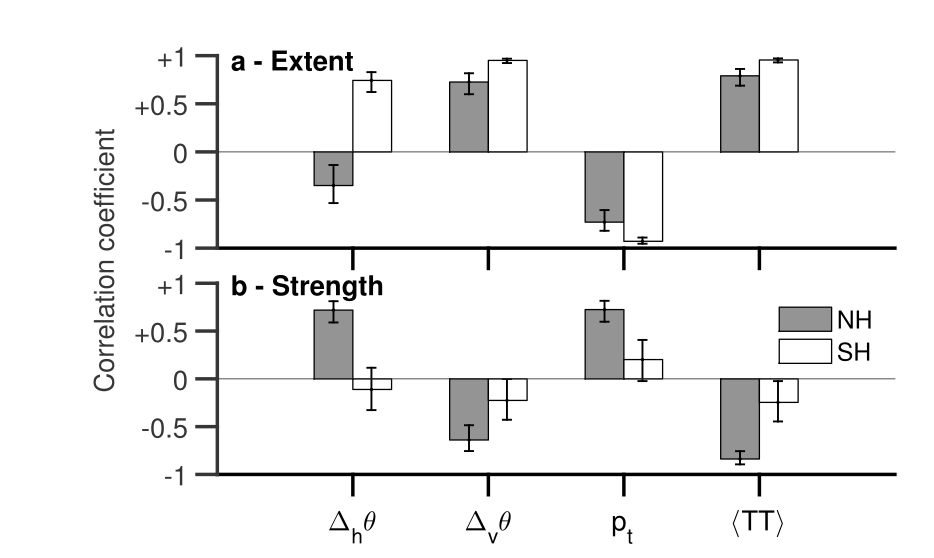
\includegraphics[width=\textwidth]{figures/dagostino_correlation.png}
    \end{figure}
\end{frame}

\begin{frame}
    \frametitle{Equinox as annual mean}
    \begin{figure}
        \centering
        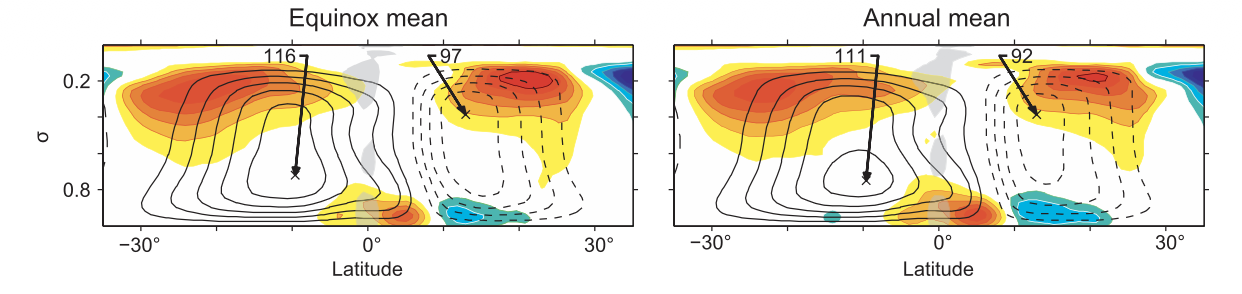
\includegraphics[width=\textwidth]{figures/equinox_mean_levine_schneider2010.png}
        \caption{Levine \& Schneider 2010}
    \end{figure}
\end{frame}

\begin{frame}
    \frametitle{Eddy fluxes}
    \begin{figure}
        \centering
        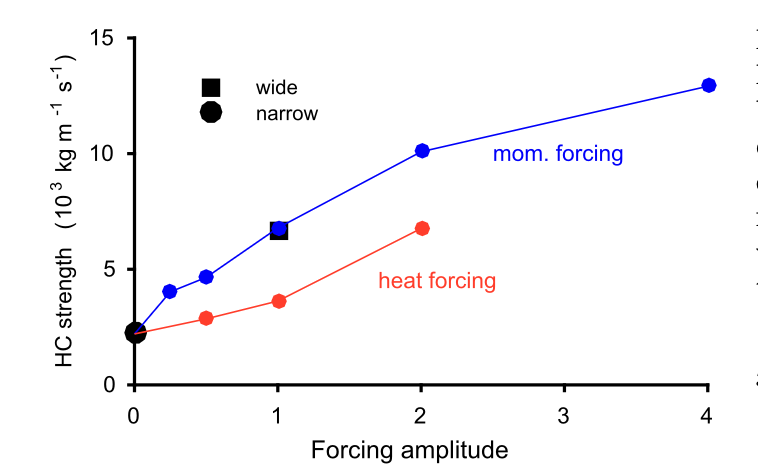
\includegraphics[width=\textwidth]{figures/strength_forcing_Singh.png}
        \caption{Singh et al. 2017}
    \end{figure}
\end{frame}

\begin{frame}
    \frametitle{Atmospheric Study Project Colloquium - 02.02.2026}
    \begin{itemize}
        \item Investigating the strengthening of the Hadley cell under tropospheric-only CO$_2$ forcing
        \item The strengthening of the Hadley circulation (cell) driven by CO2 forcing confined to the troposphere  
        \item The impact of tropospheric versus stratospheric CO$_2$ forcing on the Hadley cell 
    \end{itemize}
\end{frame}

\begin{frame}
    \begin{itemize}
        \item Motivate and explain your topic!
        \item Present the state-of-art concerning your topic: What is already known? Which results are already published? Are there publications of special relevance for you, e.g. by serving partly as a blue print?
        \item Which research gap do you want to fill? What are the innovations? What are your specific research questions and/or hypothesis?
        \item Which tools, methods, data etc. do you plan to use?
        \item Outline your workplan!
        \item (If possible, you can also present first preliminary results.) 
    \end{itemize}
\end{frame}


\backupbegin

\backupend
\end{document}
